% LaTeX mintafájl szakdolgozat és diplomamunkáknak az
% SZTE Informatikai Tanszékcsoportja által megkövetelt
% formai követelményeinek megvalósításához
% Modositva: 2011.04.28 Nemeth L. Zoltan
% A fájl használatához szükséges a magyar.ldf 2005/05/12 v1.5-ös vagy későbbi verziója
% ez letölthető a http://www.math.bme.hu/latex/ weblapról, a magyar nyelvű szedéshez
% Hasznos információk, linekek, LaTeX leirasok a www.latex.lap.hu weboldalon vannak.
%


\documentclass[12pt]{report}

%Magyar nyelvi támogatás (Babel 3.7 vagy későbbi kell!)
\def\magyarOptions{defaults=hu-min}
\usepackage[magyar]{babel}

%Az ékezetes betűk használatához:
\usepackage{t1enc}% ékezetes szavak automatikus elválasztásához
\usepackage[utf8]{inputenc}% ékezetes szavak beviteléhez

% A formai kovetelmenyekben megkövetelt Times betűtípus hasznalata:
\usepackage{times}

%Az AMS csomagjai
\usepackage{amsmath}
\usepackage{amssymb}
\usepackage{amsthm}

%A fejléc láblécek kialakításához:
\usepackage{fancyhdr}

%Természetesen további csomagok is használhatók,
%például ábrák beillesztéséhez a graphix és a psfrag,
%ha nincs rájuk szükség természetesen kihagyhatók.
\usepackage{graphicx}
\usepackage{psfrag}

\usepackage{setspace}

\usepackage{listings}
\usepackage{color}
\definecolor{myCommentColorGreen}{RGB}{0,128,0}
\definecolor{myLineNumberGray}{RGB}{128,128,128}
\lstset{ %
%    backgroundcolor=\color{white},   % choose the background color; you must add  \usepackage{color} or \usepackage{xcolor}
    basicstyle=\footnotesize,        % the size of the fonts that are used for    the code
%    breakatwhitespace=false,         % sets if automatic breaks should only      happen at whitespace
    breaklines=true,                 % sets automatic line breaking          captionpos=b,                    % sets the caption-position to          bottom
    commentstyle=\color{myCommentColorGreen},    % comment style
%    deletekeywords={...},            % if you want to delete keywords              from the given language
%    escapeinside={\%*}{*)},          % if you want to add LaTeX                within your code
%    extendedchars=true,              % lets you use non-ASCII                  characters; for 8-bits encodings only, does not work with                  UTF-8
     frame=leftline, %single,                    % adds a frame around the                    code
%    keepspaces=true,                 % keeps spaces in text,                      useful for keeping indentation of code (possibly needs                      columns=flexible)
    keywordstyle=\color{blue},       % keyword style
    language=C++,%Octave,                 % the language of                          the code
%    morekeywords={*,...},            % if you want to                            add more keywords to the set
    numberfirstline=true,
    numbers=left,                    % where to put                              the line-numbers; possible values are (none, left, right)
    numbersep=10pt,                   % how far theline-numbers are from the code
    numberstyle=\tiny\color{myLineNumberGray}, % the stylethat is used for the line-numbers
%    name=\thelstnumber, %
%    rulecolor=\color{black},         % if notset, the frame-color may be changed online-breaks within not-black text (e.g.comments (green here))
%    showspaces=false,                % showspaces everywhere adding particularunderscores; it overrides'showstringspaces'
%    showstringspaces=false,          %underline spaces within strings only
%    showtabs=false,                  %show tabs within strings addingparticular underscores
%    stepnumber=2,                    %the step between two line-numbers.If it's 1, each line will benumbered
%    stringstyle=\color{mymauve},     % string literal style
    tabsize=4,                       %   % sets default tabsize to 2    spaces
%    title=\lstname                   %     % show the filename of     files included with     \lstinputlisting; also try     caption instead of title
}

%Tételszerű környezetek definiálhatók, ezek most fejezetenkent egyutt szamozodnak, pl.
\newtheorem{tét}{Tétel}[chapter]
\newtheorem{defi}[tét]{Definíció}
\newtheorem{lemma}[tét]{Lemma}
\newtheorem{áll}[tét]{Állítás}
\newtheorem{köv}[tét]{Következmény}

%Ha a megjegyzések és a példak szövegét nem akarjuk dőlten szedni, akkor
%az alábbi parancs után kell őket definiální:
\theoremstyle{definition}
\newtheorem{megj}[tét]{Megjegyzés}
\newtheorem{pld}[tét]{Példa}

%Margók:
\hoffset -1in
\voffset -1in
\oddsidemargin 35mm
\textwidth 150mm
\topmargin 15mm
\headheight 10mm
\headsep 5mm
\textheight 237mm




\begin{document}

%A FEJEZETEK KEZDŐOLDALAINAK FEJ ÉS LÁBLÉCE:
%a plain oldalstílust kell átdefiniálni, hogy ott ne legyen fejléc:
\fancypagestyle{plain}{%
%ez mindent töröl:
\fancyhf{}
% a láblécbe jobboldalra kerüljön az oldalszám:
\fancyfoot[R]{\thepage}
%elválasztó vonal sem kell:
\renewcommand{\headrulewidth}{0pt}
}

%A TÖBBI OLDAL FEJ ÉS LÁBLÉCE:
\pagestyle{fancy}
\fancyhf{}
\fancyhead[L]{A diplomamunka címe}
\fancyfoot[R]{\thepage}


%A címoldalra se fej- se lábléc nem kell:
\thispagestyle{empty}

\begin{center}
\vspace*{1cm}
{\Large\bf Szegedi Tudományegyetem}

\vspace{0.5cm}

{\Large\bf Informatikai Tanszékcsoport}

\vspace*{3.8cm}


{\LARGE\bf A diplomamunka címe}


\vspace*{3.6cm}

{\Large Diplomamunka}
% vagy {\Large Szakdolgozat}

\vspace*{4cm}

%Értelemszerűen megváltoztatandó:
{\large
\begin{tabular}{c@{\hspace{4cm}}c}
\emph{Készítette:}     &\emph{Témavezető:}\\
\bf{Ledán Szilárd}  &\bf{Dr. Kiss Ákos}\\
informatika szakos     &adjunktus\\
hallgató&
\end{tabular}
}

\vspace*{2.3cm}

{\Large
Szeged
\\
\vspace{2mm}
2014
}
\end{center}

% 1.5-ös sorköz:
% ezt javasolják:  \linespread{1.25}
% és ez bevált, de ehhez kellett a \usepackage{setspace} csomag betöltése.
\onehalfspacing

%A tartalomjegyzék:
\tableofcontents

%A \chapter* parancs nem ad a fejezetnek sorszámot
\chapter*{Feladatkiírás}
%A tartalomjegyzékben mégis szerepeltetni kell, mint szakasz(section) szerepeljen:
\addcontentsline{toc}{section}{Feladatkiírás}

A témavezető által megfogalmazott feladatkiírás. Önálló oldalon szerepel.

\chapter*{Tartalmi összefoglaló}
\addcontentsline{toc}{section}{Tartalmi összefoglaló}

A tartalmi összefoglalónak tartalmaznia kell (rövid, legfeljebb egy oldalas, összefüggő megfogalmazásban)
a következőket: a téma megnevezése, a megadott feladat megfogalmazása - a feladatkiíráshoz viszonyítva-,
a megoldási mód, az alkalmazott eszközök, módszerek, az elért eredmények, kulcsszavak (4-6 darab).

Az összefoglaló nyelvének meg kell egyeznie a dolgozat nyelvével. Ha a dolgozat idegen nyelven készül,
magyar nyelvű tartalmi összefoglaló készítése is kötelező (külön lapon), melynek terjedelmét a TVSZ szabályozza.


\chapter*{Bevezetés}
\addcontentsline{toc}{section}{Bevezetés}

Itt kezdődik a bevezetés, mely nem kap sorszámot.



\chapter{Egy találó cím}

Ez pedig már az első fejezet, ...

\section{Alcím}
Ebben alfejezetek is lehetnek

\subsection{Al-al cím}
Sőt al-al fejezetek is.

\subsection{Másik}
Na lássunk egy másodikat is.

\subsection{Harmadik}
Meg egy harmadikat is.

\section{Mindjárt vége a fejezetnek}
Tényleg, itt valóban vége.


\chapter{Hosszú}
\section{Részletek}
Ebbe a fejezetbe pedig írunk sok sok szöveget. Szöveg, szöveg, szöveg,  szöveg, szöveg, szöveg,   szöveg, szöveg, szöveg
szöveg, szöveg, szöveg,  szöveg, szöveg, szöveg, szöveg, szöveg, szöveg, szöveg, szöveg, szöveg, szöveg, szöveg, szöveg,
szöveg, szöveg, szöveg, szöveg, szöveg, szöveg, szöveg, szöveg, szöveg, szöveg, szöveg, szöveg, szöveg, szöveg, szöveg,
szöveg, szöveg, szöveg, szöveg, szöveg, szöveg, szöveg, szöveg, szöveg, szöveg, szöveg, szöveg,
szöveg, szöveg, szöveg, szöveg, szöveg, szöveg, szöveg, szöveg, szöveg, szöveg, szöveg, szöveg, szöveg, szöveg, szöveg,
szöveg, szöveg, szöveg, szöveg, szöveg, szöveg, szöveg, szöveg, szöveg, szöveg, szöveg, szöveg, szöveg, szöveg, szöveg,
szöveg, szöveg, szöveg, szöveg, szöveg, szöveg, szöveg, szöveg, szöveg, szöveg, szöveg, szöveg, szöveg, szöveg, szöveg,
szöveg, szöveg, szöveg, szöveg, szöveg, szöveg, szöveg, szöveg, szöveg, szöveg, szöveg, szöveg, szöveg, szöveg, szöveg,
szöveg, szöveg, szöveg, szöveg, szöveg, szöveg, szöveg, szöveg, szöveg, szöveg, szöveg, szöveg, szöveg, szöveg, szöveg,
szöveg, szöveg, szöveg, szöveg, szöveg, szöveg, szöveg, szöveg, szöveg, szöveg, szöveg, szöveg, szöveg, szöveg, szöveg,
szöveg, szöveg, szöveg, szöveg, szöveg, szöveg, szöveg, szöveg, szöveg, szöveg, szöveg, szöveg, szöveg, szöveg, szöveg,
szöveg, szöveg, szöveg,  szöveg, szöveg, szöveg, szöveg, szöveg, szöveg, szöveg, szöveg, szöveg, szöveg, szöveg, szöveg,
szöveg, szöveg, szöveg, szöveg, szöveg, szöveg, szöveg, szöveg, szöveg, szöveg, szöveg, szöveg, szöveg, szöveg, szöveg,
szöveg, szöveg, szöveg, szöveg, szöveg, szöveg, szöveg, szöveg, szöveg, szöveg, szöveg, szöveg,
szöveg, szöveg, szöveg, szöveg, szöveg, szöveg, szöveg, szöveg, szöveg, szöveg, szöveg, szöveg, szöveg, szöveg, szöveg,
szöveg, szöveg, szöveg, szöveg, szöveg, szöveg, szöveg, szöveg, szöveg, szöveg, szöveg, szöveg, szöveg, szöveg, szöveg,
szöveg, szöveg, szöveg, szöveg, szöveg, szöveg, szöveg, szöveg, szöveg, szöveg, szöveg, szöveg, szöveg, szöveg, szöveg,
szöveg, szöveg, szöveg, szöveg, szöveg, szöveg, szöveg, szöveg, szöveg, szöveg, szöveg, szöveg, szöveg, szöveg, szöveg,
szöveg, szöveg, szöveg, szöveg, szöveg, szöveg, szöveg, szöveg, szöveg, szöveg, szöveg, szöveg, szöveg, szöveg, szöveg,
szöveg, szöveg, szöveg, szöveg, szöveg, szöveg, szöveg, szöveg, szöveg, szöveg, szöveg, szöveg, szöveg, szöveg, szöveg,
szöveg, szöveg, szöveg, szöveg, szöveg, szöveg, szöveg, szöveg, szöveg, szöveg, szöveg, szöveg, szöveg, szöveg, szöveg,
szöveg, szöveg, szöveg,  szöveg, szöveg, szöveg, szöveg, szöveg, szöveg, szöveg, szöveg, szöveg, szöveg, szöveg, szöveg,
szöveg, szöveg, szöveg, szöveg, szöveg, szöveg, szöveg, szöveg, szöveg, szöveg, szöveg, szöveg, szöveg, szöveg, szöveg,
szöveg, szöveg, szöveg, szöveg, szöveg, szöveg, szöveg, szöveg, szöveg, szöveg, szöveg, szöveg,
szöveg, szöveg, szöveg, szöveg, szöveg, szöveg, szöveg, szöveg, szöveg, szöveg, szöveg, szöveg, szöveg, szöveg, szöveg,
szöveg, szöveg, szöveg, szöveg, szöveg, szöveg, szöveg, szöveg, szöveg, szöveg, szöveg, szöveg, szöveg, szöveg, szöveg,
szöveg, szöveg, szöveg, szöveg, szöveg, szöveg, szöveg, szöveg, szöveg, szöveg, szöveg, szöveg, szöveg, szöveg, szöveg,
szöveg, szöveg, szöveg, szöveg, szöveg, szöveg, szöveg, szöveg, szöveg, szöveg, szöveg, szöveg, szöveg, szöveg, szöveg,
szöveg, szöveg, szöveg, szöveg, szöveg, szöveg, szöveg, szöveg, szöveg, szöveg, szöveg, szöveg, szöveg, szöveg, szöveg,
szöveg, szöveg, szöveg, szöveg, szöveg, szöveg, szöveg, szöveg, szöveg, szöveg, szöveg, szöveg, szöveg, szöveg, szöveg,
szöveg, szöveg, szöveg, szöveg, szöveg, szöveg, szöveg, szöveg, szöveg, szöveg, szöveg, szöveg, szöveg, szöveg, szöveg,
szöveg, szöveg, szöveg,  szöveg, szöveg, szöveg, szöveg, szöveg, szöveg, szöveg, szöveg, szöveg, szöveg, szöveg, szöveg,
szöveg, szöveg, szöveg, szöveg, szöveg, szöveg, szöveg, szöveg, szöveg, szöveg, szöveg, szöveg, szöveg, szöveg, szöveg,
szöveg, szöveg, szöveg, szöveg, szöveg, szöveg, szöveg, szöveg, szöveg, szöveg, szöveg, szöveg,
szöveg, szöveg, szöveg, szöveg, szöveg, szöveg, szöveg, szöveg, szöveg, szöveg, szöveg, szöveg, szöveg, szöveg, szöveg,
szöveg, szöveg, szöveg, szöveg, szöveg, szöveg, szöveg, szöveg, szöveg, szöveg, szöveg, szöveg, szöveg, szöveg, szöveg,

\chapter{Egyebek}

\section{Környezetek}
\begin{tét}
\label{tét-alap}
Ez itt egy tétel.
\end{tét}

%A bizonyítás \begin{proof} és \end{proof} közé kerül:
\begin{proof}
Ez pedig a bizonyítása, melyben szerepel egy képlet:
\begin{equation}
\begin{split}
E^{\text{globális}} &= \text{tét}_1\cdot E_1^{\text{elemi}}+\text{tét}_2\cdot
E_2^{\text{elemi}}+\ldots+\text{tét}_n\cdot E_n^{elemi} \\
&=E^{\text{elemi}}\left(\text{tét}_1+\text{tét}_2+\ldots+\text{tét}_n\right)\\
&=E^{\text{elemi}}\cdot\text{össztét}
\end{split}
\end{equation}
A második egyenlőségnél azt használtunk ki, hogy ...

Ezzel a bizonyítást befejeztük.
\end{proof}

\begin{defi}
\label{def-pelda}
Ez egy definíció. Számozása a tételekkel együtt történik.
\end{defi}

\begin{áll}
A követekező négy állítás egymással ekvivalens:
\label{áll-ekvivalencia}
  \begin{itemize}
  \item[(i)] $M$ és $N$ gyengén ekvivalensek.
  \item[(ii)] Minden $n$
  nemnegatív egész számra $|L_{M}\cap \Sigma_{1}^{n}|=|L_{N}\cap \Sigma_{2}^{n}|$ teljesül.
  \item[(iii)] Minden $n$ nemnegatív egész szám esetén
   létezik
  $ \pi_{n}: L_{M}\cap \Sigma_{1}^{n} \rightarrow L_{N}\cap \Sigma_{2}^{n} $ kölcsönösen egyértelmű
  leképezés.
  \item[(iv)] Minden nemnegatív $n$-re $x A^{n} y^{T}=x' A'^{n} y'^{T}$.
  \end{itemize}
\end{áll}

\begin{köv}
  Ez pedig egy következmény.
\end{köv}

\begin{pld}
  Ez lesz a példa, ezt nem szedjük dőlten.
\end{pld}

\begin{megj}
  A fejezetet pedig egy megjegyzés zárja.
\end{megj}


\section{Listák}

Ez egy felsorolás:
\begin{itemize}
    \item első
    \item második
      \subitem első
      \subitem második
    \item harmadik
    \item[$\clubsuit$]  saját jel is alkalmazható
\end{itemize}
Ez pedig egy számozott lista:
\begin{enumerate}
            \item hétfő
            \item kedd
            \item szerda
\end{enumerate}

%Oldaltörést is alkalmazhatunk
\pagebreak


\section{Egy táblázat és egy ábra}

A táblázat itt következik.
\begin{table}[!h]\label{strategia}
\caption{Példa stratégiatáblára a Black Jack esetében}
\begin{center}
\begin{tabular}{l||r|r|r|r|r|r|r|r|r|r}
&ász&2&3&4&5&6&7&8&9&10\\
\hline\hline
21&n&n&n&n&n&n&n&n&n&n\\
20&n&n&n&n&n&n&n&n&n&n\\
19&n&n&n&n&n&n&n&n&n&n\\
18&n&n&n&n&n&n&n&n&n&n\\
17&n&n&n&n&n&n&n&n&n&n\\
16&h&n&n&n&n&n&h&h&b&b\\
15&h&n&n&n&n&n&h&h&h&b\\
14&h&n&n&n&n&n&h&h&h&b\\
13&h&n&n&n&n&n&h&h&h&h\\
12&h&n&n&n&n&n&h&h&h&h\\
11&h&D&D&D&D&D&D&D&D&h\\
\end{tabular}
\end{center}
\end{table}

Lássunk egy ábrát is!
\begin{figure}[!h]
\unitlength 8mm
\begin{center}
\begin{picture}(8,6)
\thicklines
\multiput(0,1)(0,1){2}{\line(1,0){5}}
\multiput(3,0)(1,0){2}{\line(0,1){6}}
\multiput(1,0)(1,0){2}{\line(0,1){1}}
\multiput(6,0)(1,0){2}{\line(0,1){5}}
\multiput(0,1)(1,0){3}{\line(0,1){1}}
\multiput(2,4)(3,0){3}{\line(0,1){1}}
\multiput(3,0)(0,3){3}{\line(1,0){1}}
\multiput(6,0)(0,1){4}{\line(1,0){1}}
\multiput(7,2)(0,1){2}{\line(1,0){1}}
\multiput(2,4)(0,1){2}{\line(1,0){6}}
\put(5,1){\line(0,1){1}}
\put(8,2){\line(0,1){1}}
\put(1,0){\line(1,0){1}}
\put(1,1){\makebox(1,1){\(\sphericalangle\)}}
\put(7,2){\makebox(1,1){\(\$\)}}
\end{picture}
\end{center}
\caption{\label{labirintus}Labirintus bejárása}
\end{figure}

%laptörés:
\newpage

Külön fájlban elkészített grafika beillesztését a \ref{abra-automata} ábra szemlélteti.
\begin{figure}[h]
\centering
%A psfrag csomag használatával a (encapsulated)postcript abra feliratait LaTeX koddal helyettesíthatjük:
\psfrag{a}[c][c]{$q_0$}
\psfrag{b}[c][c]{$q_1$}
\psfrag{c}[c][c]{$q_2$}
\psfrag{d}[c][c]{$q_3$}
\psfrag{e}[c][c]{$q_4$}
\psfrag{f}[c][c]{$q_5$}
\psfrag{g}[c][c]{$q_6$}
\psfrag{h}[c][c]{$q_7$}
\psfrag{0}[c][c]{$a_{0}$}
\psfrag{9}[c][c]{$a_{9}$}
\psfrag{3}[c][c]{$a_{3}$}
\psfrag{12}[c][c]{$a_{12}$}
\psfrag{15}[c][c]{$a_{15}$}
%Garfika belillesztese, "scale2 a nagyitas/kicinyites merteke, itt 80%.
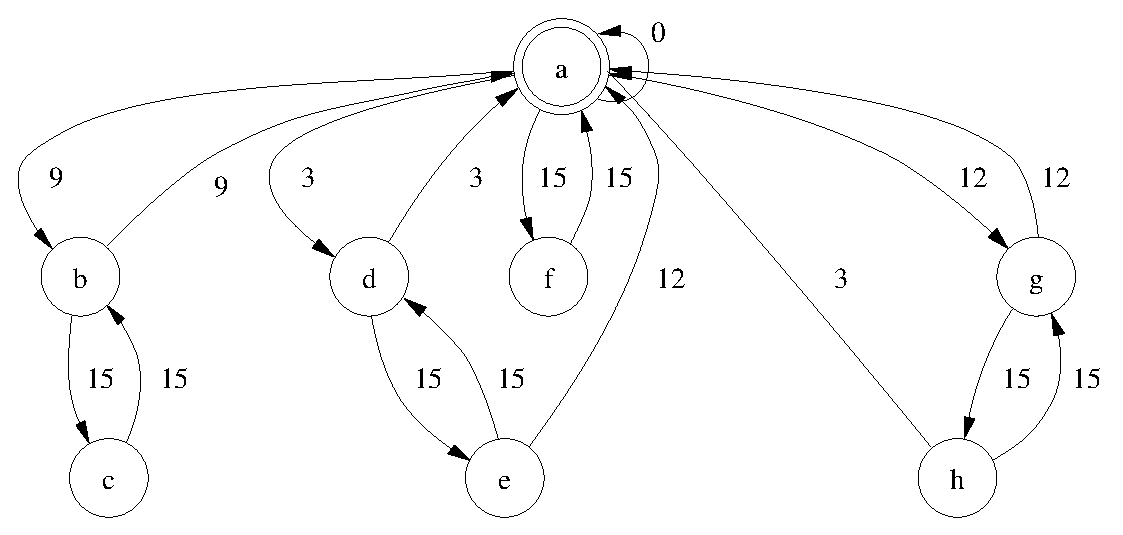
\includegraphics[scale=0.8]{abra.eps}
\caption{\label{abra-automata} A $4\times m$-es tábla lefedéseinek mátrixreprezentációit felismerő automata}
\end{figure}


\begin{figure}[h]
\centering
%%A psfrag csomag használatával a (encapsulated)postcript abra feliratait LaTeX koddal helyettesíthatjük:
\psfrag{t}[c][c]{$q_0$}
%\psfrag{b}[c][c]{$q_1$}
%\psfrag{c}[c][c]{$q_2$}
%\psfrag{d}[c][c]{$q_3$}
%\psfrag{e}[c][c]{$q_4$}
%\psfrag{f}[c][c]{$q_5$}
%\psfrag{g}[c][c]{$q_6$}
%\psfrag{h}[c][c]{$q_7$}
%\psfrag{0}[c][c]{$a_{0}$}
%\psfrag{9}[c][c]{$a_{9}$}
%\psfrag{3}[c][c]{$a_{3}$}
%\psfrag{12}[c][c]{$a_{12}$}
%\psfrag{15}[c][c]{$a_{15}$}
%%Garfika belillesztese, "scale2 a nagyitas/kicinyites merteke, itt 80%.
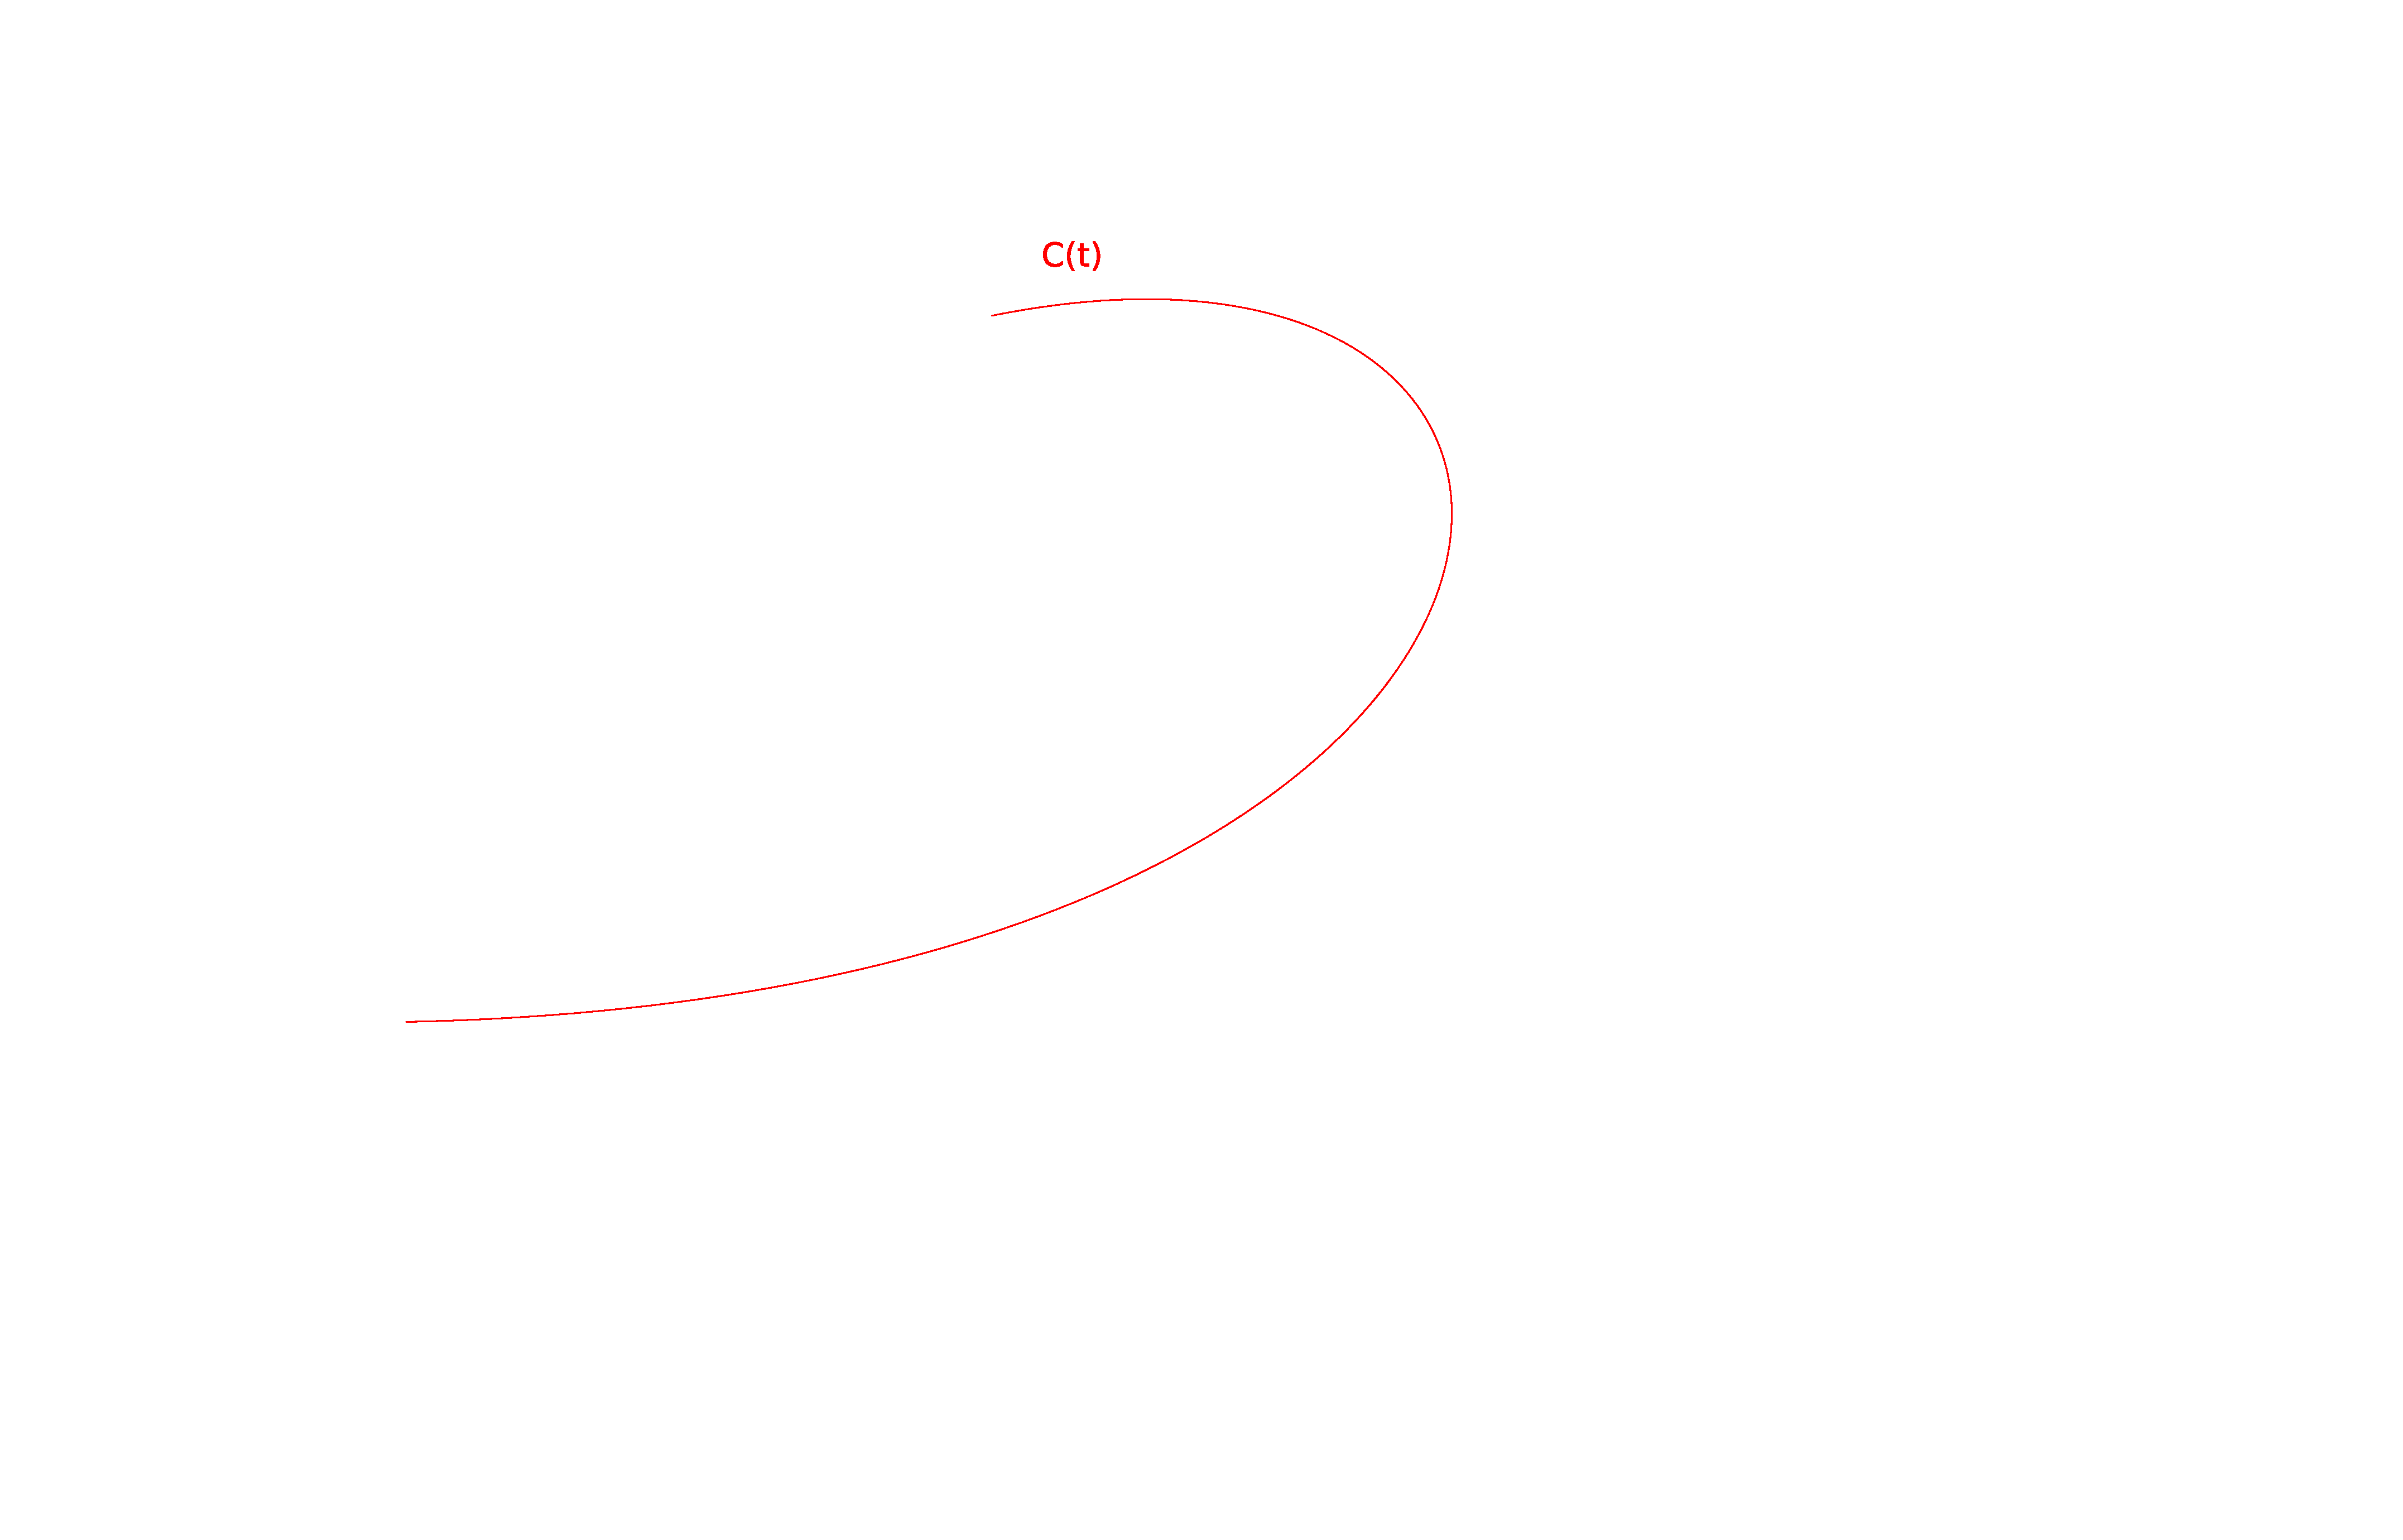
\includegraphics[scale=0.3]{bezier.eps}
\caption{\label{abra-automata} A $4\times m$-es tábla lefedéseinek mátrixreprezentációit felismerő automata}
\end{figure}


\chapter{Függelék}

\section{A program forráskódja}



\lstinputlisting[linerange={4-8}, firstnumber=4]{../../code/WebKitGL2D.git_rm/Source/WebCore/platform/graphics/gl2d/TrapezoidBuilderGL2D.cpp}
\lstinputlisting[linerange={1-112}]{../../code/WebKitGL2D.git_rm/Source/WebCore/platform/graphics/gl2d/TrapezoidBuilderGL2D.cpp}
\lstinputlisting[linerange={4-12}]{../../code/WebKitGL2D.git_rm/Source/WebCore/platform/graphics/gl2d/TrapezoidBuilderGL2D.cpp}
\begin{lstlisting}
\end{lstlisting}
A függelékbe kerülhetnek a hosszú táblázatok, vagy mondjuk egy programlista:
% A verbatim kornyezet hasznalatanal ügyeljünk rá, hogy az editor a szóközöjket át ne írja tab karakterekre!
\begin{verbatim}
   while (ujkmodosito[i]<0)
   {
      if (ujkmodosito[i]+kegyenletes[i]<0)
      {
         j=i+1;
         while (j<14)
         if (kegyenletes[i]+ujkmodosito[j]>-1) break;
         else j++;
         temp=ujkmodosito[j];
         for (l=i;l<j;l++) ujkmodosito[l+1]=ujkmodosito[l];
         ujkmodosito[i]=temp;
      }
      i++;
   }
\end{verbatim}


\chapter*{Nyilatkozat}
%Egy üres sort adunk a tartalomjegyzékhez:
\addtocontents{toc}{\ }
\addcontentsline{toc}{section}{Nyilatkozat}
%\hspace{\parindent}

% A nyilatkozat szövege más titkos és nem titkos dolgozatok esetében.
% Csak az egyik típusú nyilatkozatnak kell a dolgozatban szerepelni
% A pontok helyére az adatok értelemszerűen behelyettesítendők és
% a szakdolgozat /diplomamunka szó megfelelően kiválasztandó.


% A nyilatkozat szövege TITKOSNAK NEM MINŐSÍTETT dolgozatban a következő:
% A pontokkal jelölt szövegrészek értelemszerűen a szövegszerkesztőben és
% nem kézzel helyettesítendők:

\noindent
Alulírott \makebox[4cm]{\dotfill} szakos hallgató, kijelentem, hogy a dolgozatomat a Szegedi Tudományegyetem, Informatikai Tanszékcsoport \makebox[4cm]{\dotfill} Tanszékén készítettem, \makebox[4cm]{\dotfill} diploma megszerzése érdekében.

Kijelentem, hogy a dolgozatot más szakon korábban nem védtem meg, saját munkám eredménye, és csak a hivatkozott forrásokat (szakirodalom, eszközök, stb.) használtam fel.

Tudomásul veszem, hogy szakdolgozatomat / diplomamunkámat a Szegedi Tudományegyetem Informatikai Tanszékcsoport könyvtárában, a helyben olvasható könyvek között helyezik el.

\vspace*{2cm}

\begin{tabular}{lc}
Szeged, \today\
\hspace{2cm} & \makebox[6cm]{\dotfill} \\
& aláírás \\
\end{tabular}


\vspace*{4cm}

%A nyilatkozat szövege TITKOSNAK MINŐSÍTETT dolgozatban a következő:

\noindent
Alulírott \makebox[4cm]{\dotfill} szakos hallgató, kijelentem, hogy a dolgozatomat a Szegedi Tudományegyetem, Informatikai Tanszékcsoport \makebox[4cm]{\dotfill} Tanszékén készítettem, \makebox[4cm]{\dotfill} diploma megszerzése érdekében.

Kijelentem, hogy a dolgozatot más szakon korábban nem védtem meg, saját munkám eredménye, és csak a hivatkozott forrásokat (szakirodalom, eszközök, stb.) használtam fel.

Tudomásul veszem, hogy szakdolgozatomat / diplomamunkámat a TVSZ 4. sz. mellékletében leírtak szerint kezelik.

\vspace*{2cm}

\begin{tabular}{lc}
Szeged, \today\
\hspace{2cm} & \makebox[6cm]{\dotfill} \\
& aláírás \\
\end{tabular}





\chapter*{Köszönetnyilvánítás}
\addcontentsline{toc}{section}{Köszönetnyilvánítás}

Ezúton szeretnék köszönetet mondani \textbf{X. Y-nak} ezért és ezért \ldots


%% Az itrodalomjegyzek keszitheto a BibTeX segedprogrammal:
%\bibliography{diploma}
%\bibliographystyle{plain}

%VAGY "kézzel" a következő módon:

\begin{thebibliography}{9}
%10-nél kevesebb hivatkozás esetén

%\begin{thebibliography}{99}
% 10-nél több hivatkozás esetén

\addcontentsline{toc}{section}{Irodalomjegyzék}

%Elso szerzok vezetekneve alapjan ábécérendben rendezve.


%folyóirat cikk: szerzok(k), a folyóirat neve kiemelve,
%az evfolyam felkoveren, zarojelben az evszam, vegul az oldalszamok es pont.
\bibitem{Gischer}
J. L. Gischer,
The equational theory of pomsets.
\emph{Theoret. Comput. Sci.}, \textbf{61}(1988), 199--224.

%könyv (szerzo(k), a könyv neve kiemelve, utana a kiado, a kiado szekhelye, az evszam es pont.)
\bibitem{Pin}
J.-E. Pin,
\emph{Varieties of Formal Languages},
Plenum Publishing Corp., New York, 1986.





\end{thebibliography}




\end{document}
